% ============================================================================
%  VAJRA - project synopsis report
%  Build:  xelatex report.tex   (run twice)
%  Fonts:  Charter (text), Avenir Next (headings), Menlo (code).
%          Falls back to TeX Gyre / Latin Modern if those are not installed.
% ============================================================================
\documentclass[10pt,a4paper]{article}

% ---- fill these in ---------------------------------------------------------
\newcommand{\authorname}{Karthik G}
\newcommand{\rollno}{CB.SC.U4CSE23270}
% ----------------------------------------------------------------------------

\usepackage[a4paper,top=1.5cm,bottom=1.5cm,left=1.65cm,right=1.65cm,
            headsep=0.35cm,footskip=0.7cm]{geometry}
\usepackage{fontspec}
\usepackage{microtype}
\usepackage{xcolor}
\usepackage{graphicx}
\usepackage{booktabs}
\usepackage{array}
\usepackage{enumitem}
\usepackage{titlesec}
\usepackage{fancyhdr}
\usepackage{caption}
\usepackage{listings}
\usepackage{tikz}
\usepackage[colorlinks=true,linkcolor=accent,urlcolor=accent]{hyperref}
\hypersetup{pdftitle={Vajra: project report},pdfauthor={Karthik G},pdfsubject={Blockchain integrity layer for a secure telemetry exchange}}

% ---- fonts: the "font change" ---------------------------------------------
\IfFontExistsTF{Charter}{%
  \setmainfont{Charter}}{%
  \IfFontExistsTF{TeX Gyre Pagella}{\setmainfont{TeX Gyre Pagella}}{\relax}}
\IfFontExistsTF{Avenir Next}{%
  \newfontfamily\headfont{Avenir Next}[BoldFont={Avenir Next Demi Bold},Ligatures=TeX]}{%
  \IfFontExistsTF{TeX Gyre Heros}{\newfontfamily\headfont{TeX Gyre Heros}}{\newcommand{\headfont}{\sffamily}}}
\IfFontExistsTF{Menlo}{%
  \setmonofont{Menlo}[Scale=0.80]}{%
  \IfFontExistsTF{TeX Gyre Cursor}{\setmonofont{TeX Gyre Cursor}[Scale=0.9]}{\relax}}

% ---- colours ---------------------------------------------------------------
\definecolor{accent}{HTML}{1F3A5F}
\definecolor{ember}{HTML}{D9531E}
\definecolor{iris}{HTML}{5B4BC4}
\definecolor{ink}{HTML}{2B2B2B}
\definecolor{mist}{HTML}{EEF2F7}

% ---- text shape ------------------------------------------------------------
\setlength{\parindent}{0pt}
\setlength{\parskip}{2pt}
\linespread{1.03}
\setlist[itemize]{label={\color{accent}\raisebox{0.18ex}{\rule{0.38em}{0.38em}}},
                  leftmargin=1.05em, itemsep=1.2pt, topsep=1.5pt, parsep=0pt, partopsep=0pt}
\setlist[enumerate]{leftmargin=1.45em, itemsep=1.2pt, topsep=1.5pt, parsep=0pt}

\titleformat{\section}{\headfont\bfseries\large\color{accent}}{\thesection}{0.55em}{}
  [{\vspace{1.5pt}\color{accent!30}\titlerule[0.5pt]}]
\titlespacing*{\section}{0pt}{9pt}{4pt}
\captionsetup{font=small,labelfont={bf,color=accent},skip=3pt}

\newcommand{\code}[1]{\texttt{#1}}
\newcommand{\cat}{\ensuremath{\mathbin{\Vert}}}
\newcommand{\go}{\ensuremath{\rightarrow}}

\pagestyle{fancy}
\fancyhf{}
\renewcommand{\headrulewidth}{0pt}
\fancyfoot[L]{\headfont\scriptsize\color{ink!70} Vajra \textbullet\ project report}
\fancyfoot[R]{\headfont\scriptsize\color{ink!70} \thepage}

\lstset{basicstyle=\ttfamily\fontsize{6.25}{7.6}\selectfont, columns=fixed,
        showstringspaces=false, backgroundcolor=\color{mist}, frame=single, rulecolor=\color{accent!30},
        framesep=3pt, framerule=0.4pt, xleftmargin=0pt, aboveskip=0pt, belowskip=0pt}

% ---- tikz styles -----------------------------------------------------------
\usetikzlibrary{arrows.meta,positioning,fit,backgrounds,calc}
\tikzset{
  box/.style={draw=ink!60, rounded corners=2.5pt, fill=white, align=center,
              inner sep=3pt, font=\headfont\footnotesize, minimum height=1.0cm, text width=3.75cm},
  arr/.style={-{Stealth[length=4pt]}, draw=ink!75, line width=0.6pt},
  darr/.style={{Stealth[length=4pt]}-{Stealth[length=4pt]}, draw=ink!75, line width=0.6pt},
  lbl/.style={font=\headfont\scriptsize, text=ink!85, fill=white, inner sep=1pt},
  small/.style={draw=ink!55, rounded corners=1.5pt, fill=white, font=\headfont\scriptsize,
                inner sep=2.5pt, minimum height=0.6cm, minimum width=1.4cm, align=center},
}

\begin{document}

% ============================== title block =================================
\begin{center}
  {\headfont\bfseries\fontsize{22}{24}\selectfont\color{accent}VAJRA\par}
  \vspace{1pt}
  {\headfont\large Secure satellite telemetry exchange with a blockchain integrity layer\par}
  \vspace{3pt}
  {\headfont\footnotesize\color{ink!80} Project Report \ \textbullet\ \authorname\ \textbullet\ \rollno\par}
\end{center}
\vspace{-4pt}
\noindent\fcolorbox{accent!35}{mist}{%
\begin{minipage}{\dimexpr\linewidth-2\fboxsep-2\fboxrule\relax}
\small
Vajra lets ground stations and operators share satellite telemetry files without having to trust the
network or the storage. Files are encrypted in chunks, signed, and released only after multi-factor
login and a role check. This report is about the part we added on top: a blockchain layer that lets us
\emph{prove} that a stored file or an audit record has not been quietly changed, even by someone who
controls the database.
\end{minipage}}

% ============================== 1 ============================================
\section{Why}
\begin{itemize}
  \item Telemetry is sensitive \emph{and} consequential: one altered file can mislead a mission, so people need proof
        that data is unchanged, not only that it is hidden.
  \item Encryption, MFA and roles keep outsiders out. They say much less about a compromised admin account or database.
  \item Our own integrity check had a blind spot. It compared a file's chunks with hashes stored \emph{in the same database}.
        Anyone who can edit one can edit the other, recompute the hashes, and every check still passes.
  \item The fix is a reference the attacker cannot reach. We put small fingerprints on a blockchain, where records cannot be
        edited afterwards, and compare against those.
\end{itemize}

% ============================== 2 ============================================
\section{What Vajra already did}
\begin{itemize}
  \item \textbf{Stack:} React and Vite on the front end, FastAPI (Python) on the back end, Supabase for Postgres,
        object storage and authentication.
  \item \textbf{Upload path:} choose a classification (Public, Mission Logs, Top Secret) \go\ split into 512~KB chunks
        \go\ seal each chunk with AES-256-GCM \go\ SHA-256 of every chunk \go\ optional Ed25519 signature over the chunk
        hashes and a file manifest.
  \item \textbf{Identity:} email and password, then a six-digit emailed code (MFA); JWT sessions; roles (admin, manager,
        engineer, staff) plus attribute checks on classification.
  \item \textbf{Keys:} every user gets an Ed25519 pair, with the private key encrypted under a vault password (PBKDF2).
        File keys either go into the vault (password and MFA to get them back) or, in manual mode, come back as a numbered
        key file such as \code{vajra-key-0007.txt} that the user selects when downloading.
  \item \textbf{Audit:} logins, uploads, downloads and denied attempts are all logged.
\end{itemize}

\begin{figure}[!ht]
\centering
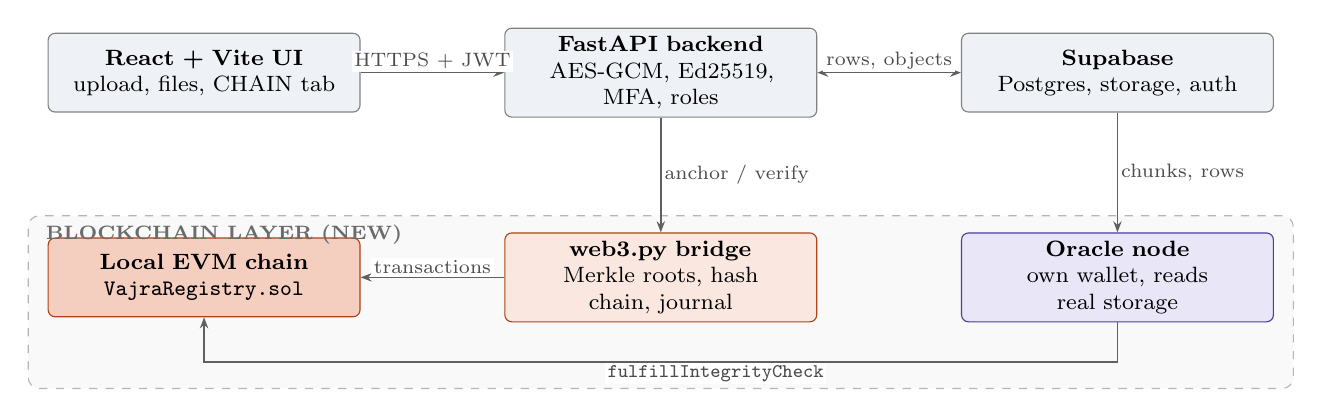
\begin{tikzpicture}
  \node[box, fill=mist] (ui)  at (0,0)    {\textbf{React + Vite UI}\\upload, files, CHAIN tab};
  \node[box, fill=mist] (api) at (5.8,0)  {\textbf{FastAPI backend}\\AES-GCM, Ed25519, MFA, roles};
  \node[box, fill=mist] (db)  at (11.6,0) {\textbf{Supabase}\\Postgres, storage, auth};
  \node[box, fill=ember!14, draw=ember!80!black] (bridge) at (5.8,-2.6) {\textbf{web3.py bridge}\\Merkle roots, hash chain, journal};
  \node[box, fill=ember!28, draw=ember!80!black] (chain)  at (0,-2.6)   {\textbf{Local EVM chain}\\\code{VajraRegistry.sol}};
  \node[box, fill=iris!14,  draw=iris!80!black]  (oracle) at (11.6,-2.6) {\textbf{Oracle node}\\own wallet, reads real storage};
  \draw[arr]  (ui)  -- node[lbl,above]{HTTPS + JWT} (api);
  \draw[darr] (api) -- node[lbl,above]{rows, objects} (db);
  \draw[arr]  (api) -- node[lbl,right]{anchor / verify} (bridge);
  \draw[arr]  (bridge) -- node[lbl,above]{transactions} (chain);
  \draw[arr]  (db)  -- node[lbl,right]{chunks, rows} (oracle);
  \draw[arr]  (oracle.south) -- ++(0,-0.5) -| node[lbl,pos=0.22,below]{\code{fulfillIntegrityCheck}} (chain.south);
  \begin{scope}[on background layer]
    \node[draw=ink!35, dashed, rounded corners=4pt, fill=ink!3, inner xsep=7pt, inner ysep=6pt,
          fit={(bridge)(chain)(oracle)(0,-3.8)}] (layer) {};
  \end{scope}
  \node[font=\headfont\scriptsize\bfseries, text=ink!70, anchor=north west] at (layer.north west) {\ BLOCKCHAIN LAYER (NEW)};
\end{tikzpicture}
\caption{Architecture. The top row is the original system; the dashed box is what we added.}
\end{figure}

% ============================== 3 ============================================
\section{The blockchain layer in one page}
\begin{itemize}
  \item \textbf{What it is:} a Solidity contract, \code{VajraRegistry} (296 lines, 9 events, 13 custom errors), on an
        Ethereum-compatible local chain (Hardhat, chain ID 31337). The backend talks to it through web3.py.
  \item \textbf{Golden rule:} only fingerprints go on-chain. Files, keys, names, classifications and identities never do.
\end{itemize}
\begin{center}
\small
\begin{tabular}{@{}p{8.0cm}p{8.0cm}@{}}
\toprule
\textbf{On-chain (public, permanent)} & \textbf{Never on-chain} \\
\midrule
Merkle root of a file's encrypted chunk hashes; hash of the signed manifest; SHA-256 of the file id (not the id);
audit-ledger head; oracle requests, reports and alarms
& File contents or keys; filenames and classification levels; user identities or emails; private signing keys \\
\bottomrule
\end{tabular}
\end{center}
\begin{enumerate}
  \item \textbf{Upload:} chunk hashes are folded into one Merkle root.
  \item \textbf{Anchor:} \code{anchorFile} writes the root and a manifest hash to the contract, once.
  \item \textbf{CHECK:} the backend recomputes the root from the database and compares it with the chain.
  \item \textbf{Oracle:} every 60 seconds the contract asks for a fresh look at real storage, and raises an alarm on a mismatch.
  \item \textbf{Ledger:} an admin can pin the head of the audit log on-chain so history cannot be rolled back.
\end{enumerate}

% ============================== 4 ============================================
\section{Core mechanisms}
\begin{itemize}
  \item \textbf{Merkle tree.} Leaf $=\mathrm{SHA256}(\texttt{0x00}\cat \mbox{index}\cat \mbox{chunk hash})$,
        node $=\mathrm{SHA256}(\texttt{0x01}\cat\min\cat\max)$. One 32-byte root commits to every chunk \emph{and} its position,
        and a single chunk can be proven with only $\log_2 n$ hashes.
  \item \textbf{Careful details.} The \texttt{0x00}/\texttt{0x01} prefixes stop a leaf from posing as an inner node, and an odd
        node is promoted, never duplicated, which avoids the duplicate-leaf ambiguity in Bitcoin's tree (CVE-2012-2459).
  \item \textbf{One byte layout, two languages.} The same hashing runs in Python and in Solidity; proofs built in Python are
        verified by the contract in our tests.
  \item \textbf{Hash-chained audit ledger.} Every log entry stores $\mathrm{SHA256}(\mbox{previous hash}\cat\mbox{entry})$.
        Edit or delete any row and every hash after it breaks; the verifier names the first bad entry.
  \item \textbf{Why pin the head on-chain.} An attacker could recompute a whole forged chain. The head stored in the contract
        (sequence numbers must strictly increase) is what they cannot forge.
  \item \textbf{Contract rules.} Anchors are write-once; revoking flags a file but never deletes it; three roles (owner,
        anchorer, oracle) are enforced by modifiers; failures use custom errors; every change emits an event.
\end{itemize}

\begin{figure}[!ht]
\centering
\begin{minipage}[b]{0.52\linewidth}\centering
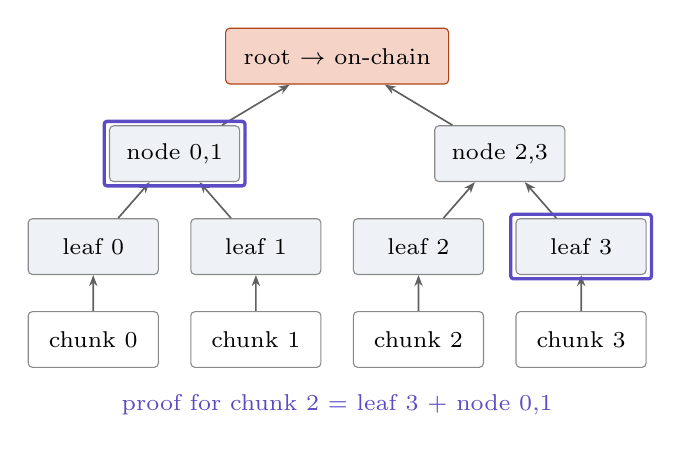
\begin{tikzpicture}[scale=1.18, transform shape]
  \foreach \i/\x in {0/0,1/1.75,2/3.5,3/5.25}{
    \node[small] (c\i) at (\x,0) {chunk \i};
    \node[small, fill=mist] (l\i) at (\x,1.0) {leaf \i};
    \draw[arr] (c\i) -- (l\i);
  }
  \node[small, fill=mist] (n01) at (0.875,2.0) {node 0,1};
  \node[small, fill=mist] (n23) at (4.375,2.0) {node 2,3};
  \node[small, fill=ember!25, draw=ember!80!black, minimum width=2.4cm] (root) at (2.625,3.05) {root $\to$ on-chain};
  \draw[arr] (l0)--(n01); \draw[arr] (l1)--(n01); \draw[arr] (l2)--(n23); \draw[arr] (l3)--(n23);
  \draw[arr] (n01)--(root); \draw[arr] (n23)--(root);
  \node[font=\headfont\scriptsize, text=iris, align=center] at (2.625,-0.7) {proof for chunk 2 = leaf 3 + node 0,1};
  \draw[iris, very thick, rounded corners=1pt] ($(l3.north west)+(-0.05,0.04)$) rectangle ($(l3.south east)+(0.05,-0.04)$);
  \draw[iris, very thick, rounded corners=1pt] ($(n01.north west)+(-0.05,0.04)$) rectangle ($(n01.south east)+(0.05,-0.04)$);
\end{tikzpicture}
\end{minipage}\hfill
\begin{minipage}[b]{0.46\linewidth}\centering
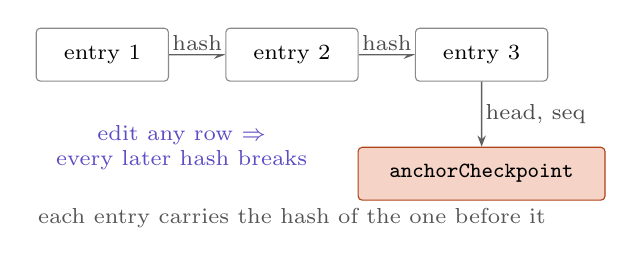
\begin{tikzpicture}[scale=1.12, transform shape]
  \node[small, minimum width=1.5cm] (e1) at (0,1.9) {entry 1};
  \node[small, minimum width=1.5cm] (e2) at (2.15,1.9) {entry 2};
  \node[small, minimum width=1.5cm] (e3) at (4.3,1.9) {entry 3};
  \draw[arr] (e1) -- node[lbl,above]{hash} (e2);
  \draw[arr] (e2) -- node[lbl,above]{hash} (e3);
  \node[small, fill=ember!25, draw=ember!80!black, minimum width=2.8cm] (cp) at (4.3,0.55) {\code{anchorCheckpoint}};
  \draw[arr] (e3) -- node[lbl,right]{head, seq} (cp);
  \node[font=\headfont\scriptsize, text=ink!80, align=center] at (2.15,0.05) {each entry carries the hash of the one before it};
  \node[font=\headfont\scriptsize, text=iris, align=center] at (0.9,0.85) {edit any row $\Rightarrow$\\every later hash breaks};
\end{tikzpicture}
\end{minipage}
\caption{Left: Merkle tree over four chunks, with the proof path for chunk 2. Right: the hash-chained audit ledger and its on-chain checkpoint.}
\end{figure}

% ============================== 5 ============================================
\section{The oracle}
\begin{itemize}
  \item \textbf{The problem:} a contract cannot read Supabase or a disk, so it cannot notice by itself that a stored file changed.
        An \emph{oracle} is the messenger that carries what it saw back on-chain.
  \item \textbf{Our flow:} the contract emits \code{IntegrityCheckRequested}; the oracle node downloads every stored chunk, reads
        the database row and recomputes the Merkle root; it answers with \code{fulfillIntegrityCheck} from its own wallet; the
        \emph{contract} compares the answer with the anchor and records Healthy or Compromised, raising \code{TamperAlarm} on a mismatch.
  \item \textbf{It reports, it does not decide.} The comparison happens inside the contract, so the oracle cannot just declare a file fine.
  \item \textbf{Separate wallets.} The anchoring wallet and the oracle wallet are different, so no single key can write a
        commitment \emph{and} vouch for it.
  \item \textbf{No false alarms.} If storage is unreachable the oracle stays silent and retries. ``Could not look'' is not
        ``found tampering''. A chunk or row that is positively gone is treated as tampering.
  \item \textbf{Honest limit:} one oracle means one point of trust (the ``oracle problem''). Production systems use several
        independent oracles and require a majority; we kept one for clarity.
\end{itemize}

\begin{figure}[!ht]
\centering
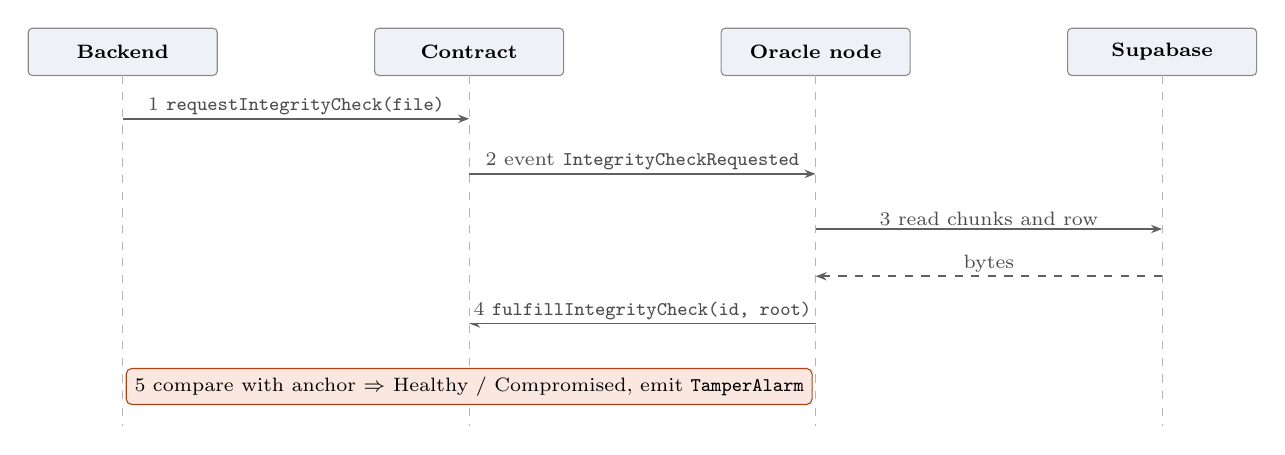
\begin{tikzpicture}[scale=1.0, transform shape]
  \foreach \n/\x/\t in {b/0/Backend, c/4.4/Contract, o/8.8/Oracle node, s/13.2/Supabase}{
    \node[small, minimum width=2.4cm, fill=mist] (h\n) at (\x,0) {\textbf{\t}};
    \draw[ink!35, dashed] (\x,-0.3) -- (\x,-4.75);
  }
  \draw[arr] (0,-0.85) -- node[lbl,above]{1\ \code{requestIntegrityCheck(file)}} (4.4,-0.85);
  \draw[arr] (4.4,-1.55) -- node[lbl,above]{2\ event \code{IntegrityCheckRequested}} (8.8,-1.55);
  \draw[arr] (8.8,-2.25) -- node[lbl,above]{3\ read chunks and row} (13.2,-2.25);
  \draw[arr,dashed] (13.2,-2.85) -- node[lbl,above]{bytes} (8.8,-2.85);
  \draw[arr] (8.8,-3.45) -- node[lbl,above]{4\ \code{fulfillIntegrityCheck(id, root)}} (4.4,-3.45);
  \node[draw=ember!80!black, fill=ember!14, rounded corners=2pt, font=\headfont\scriptsize, align=center, inner sep=3pt]
       at (4.4,-4.25) {5\ compare with anchor $\Rightarrow$ Healthy / Compromised, emit \code{TamperAlarm}};
\end{tikzpicture}
\caption{One oracle round trip. Step 5 happens inside the contract.}
\end{figure}

% ============================== 6 ============================================
\section{Making it dependable}
\begin{itemize}
  \item \textbf{Nothing extra to start.} Starting the backend launches the local node, deploys the contract (and redeploys a
        stale one, detected through a \code{version()} call), restores earlier anchors, and starts the oracle. The CHAIN tab shows the progress.
  \item \textbf{Surviving restarts.} The local chain lives in memory, so every anchor is also appended to a hash-chained journal
        (\code{chain\_journal.jsonl}). On start it is replayed, the way a node rebuilds state from history. Replay is safe to repeat,
        stops at the first edited line, and refuses to extend a corrupted journal.
  \item \textbf{Fail-open, never silent.} If the chain is down an upload still succeeds, but the file is reported as
        ``not anchored'' rather than quietly passing.
  \item \textbf{A bug we found and fixed.} The oracle re-read every past request every two seconds, and the node log grew to
        353~MB. It now remembers what it has scanned: with twelve past requests on the chain we measured zero read calls over four idle seconds, and the log stays near 3~KB.
  \item \textbf{Another catch:} unchecking ``save key to vault'' crashed the upload page (an undefined setter). Fixed while adding manual key files.
\end{itemize}

% ============================== 7 ============================================
\section{Testing and results}
\begin{center}
\small
\renewcommand{\arraystretch}{1.12}
\begin{tabular}{@{}p{3.0cm}p{9.6cm}p{2.6cm}@{}}
\toprule
\textbf{Layer} & \textbf{What is checked} & \textbf{Result} \\
\midrule
Contract (Hardhat) & roles, write-once anchors, verdicts, revocation, checkpoints, oracle request/callback & 33 of 33 pass \\
Python (unittest) & Merkle proofs for every size 1--25 at every index; hash chain under edit, delete, reorder and full recompute; journal tamper and replay & 23 of 23 pass \\
Cross-language & Python-built proofs accepted by Solidity for 1, 2, 3, 5, 8, 13 chunks; forged chunks rejected & pass \\
Oracle scenario & healthy, tampered, storage unreachable, restored (Figure~\ref{fig:evidence}) & pass \\
Restart & node killed and restarted: 3 anchors rebuilt with original roots; an edited journal replays 0 anchors & pass \\
Cost & \code{anchorFile} on the local chain & 140{,}156 gas \\
\bottomrule
\end{tabular}
\end{center}

\begin{figure}[!ht]
\centering
\begin{minipage}[t]{0.585\linewidth}
\lstinputlisting{evidence/oracle_short.txt}
\end{minipage}\hfill
\begin{minipage}[t]{0.385\linewidth}
\lstinputlisting{evidence/wallets_short.txt}
\end{minipage}
\caption{Real output from our runs. Left: the oracle scenario on an isolated local chain, using a scripted stand-in for the storage
reading so the run could not touch the real database. Right: the two wallets and their roles, and the test totals.}
\label{fig:evidence}
\end{figure}

% ============================== 8 ============================================
\section{Demo walkthrough}
\begin{itemize}
  \item \textbf{Upload, then CHECK.} The BLOCKCHAIN ANCHOR block shows the block number, transaction hash and two equal roots.
  \item \textbf{Be the attacker.} Change one chunk hash directly in Supabase. CHECK turns red (\emph{compromised}) because the
        database root no longer matches the chain.
  \item \textbf{The oracle notices on its own.} Within a minute, or on a button press, a \code{TamperAlarm} appears in the CHAIN tab.
  \item \textbf{Restore the row.} The oracle re-checks and the file turns healthy again, but the alarm stays in the history.
  \item \textbf{Ledger.} ``Verify ledger'' walks the hash chain; ``Anchor head on-chain'' pins it.
  \item \textbf{Remix IDE.} The same contract was also deployed in Remix with two accounts to show each rule one at a time: write-once
        anchors, Merkle proofs, access control, the oracle, and checkpoints.
\end{itemize}

\begin{figure}[!ht]
\centering
\IfFileExists{figures/live_check.png}{%
  \includegraphics[height=6.1cm]{figures/live_check.png}\hfill
  \IfFileExists{figures/live_oracle.png}{\includegraphics[height=6.1cm]{figures/live_oracle.png}}{}
  \caption{The running application: integrity check with its blockchain anchor block, and the oracle event feed.}
}{%
  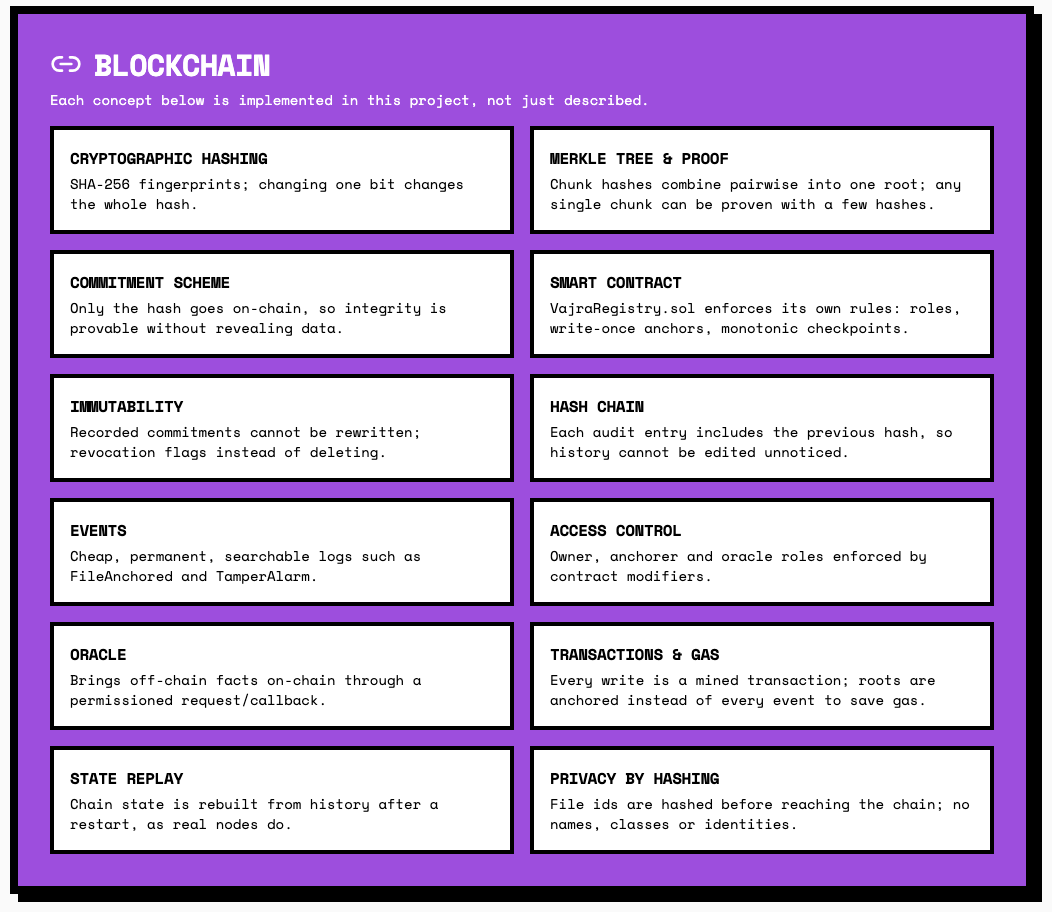
\includegraphics[width=0.485\linewidth]{figures/docs_concepts.png}\hfill
  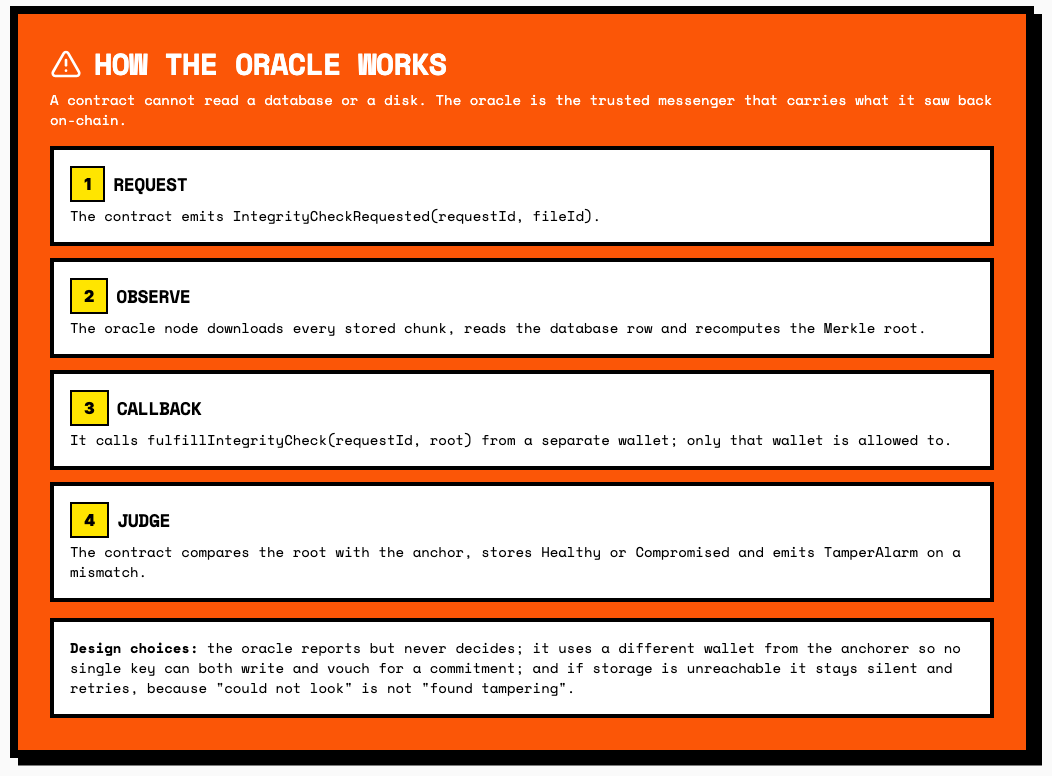
\includegraphics[width=0.485\linewidth]{figures/docs_oracle.png}
  \caption{The in-app documentation page, captured from the running frontend: the blockchain concepts and the oracle walkthrough.}
}
\end{figure}

% ============================== 9 ============================================
\section{Blockchain concepts covered}
\begin{itemize}
  \item \textbf{Implemented:} cryptographic hashing; Merkle tree and proofs; commitment scheme; smart contract (Solidity); write-once
        and append-only state; hash chain; events; role-based access control; transactions, blocks and gas; on-chain versus
        off-chain data; oracle (request and callback); state replay; privacy by hashing; digital signatures (Ed25519 manifest, hash anchored).
  \item \textbf{Deliberately not implemented:} our own consensus algorithm (the local node mines each transaction at once; on a
        public testnet it would be proof of stake), tokens, multi-signature governance, IPFS.
\end{itemize}

% ============================== 10 ===========================================
\section{Tools and technology}
\begin{itemize}
  \item \textbf{Chain:} Solidity 0.8.24, Hardhat 2, Chai and ethers v6 for tests, Remix IDE for the contract demo, web3.py 7.
  \item \textbf{Application:} Python 3.11, FastAPI, Supabase, React 19, Vite 7, Tailwind 4; about 2{,}500 new lines across contract, tests,
        backend and UI.
  \item \textbf{Report:} LaTeX (XeLaTeX); figures drawn in TikZ; screenshots and terminal output captured from the running project.
\end{itemize}

% ============================== 11 ===========================================
\section{Limitations and next steps}
\begin{itemize}
  \item \textbf{Local chain.} The same contract deploys unchanged to a public testnet such as Sepolia; we have not deployed there.
  \item \textbf{One oracle.} Next step: several oracles with a quorum.
  \item \textbf{Earlier files.} Files uploaded before the blockchain layer show ``not anchored'' until an admin anchors them.
  \item \textbf{Trust in the journal.} Replay trusts a local file. It is hash-chained so edits are caught, but a public chain is the real answer.
  \item \textbf{Oracle sweeps cost gas} on a public chain, so the interval would be lengthened there.
  \item \textbf{Session tokens.} The backend reads claims from the JWT; verifying its signature server-side is a worthwhile hardening step.
\end{itemize}

% ============================== 12 ===========================================
\section{Conclusion}
\begin{itemize}
  \item We started with a system that protected files from outsiders and trusted its own database. We ended with one that can
        \emph{prove} a file or a log has not been altered, and notices if it has.
  \item The blockchain layer is small on purpose: a 296-line contract, fingerprints only, and a clear split between what the
        chain knows and what it is told.
  \item It is tested at every level, from single contract rules to a full tamper-detect-recover scenario, and it starts itself.
\end{itemize}

\vspace{2pt}
{\footnotesize\color{ink!80}\textbf{References.}\ (1) R.~Merkle, ``A digital signature based on a conventional encryption function'', CRYPTO 1987.
(2) CVE-2012-2459, Bitcoin Merkle-tree duplicate-leaf weakness. (3) Solidity 0.8 and Hardhat documentation.
(4) NIST SP 800-63B, authenticator assurance levels.\par}

\end{document}
